\documentclass[12pt,letterpaper,english,bibliography=totocnumbered, abstract=on]{scrartcl}

\usepackage{indentfirst}
\usepackage{appendix}
%\usepackage{fullpage}
%\usepackage{subfiles}
\usepackage[T1]{fontenc}
\usepackage[latin9]{inputenc}
\usepackage{color}
\usepackage{babel}
\usepackage{verbatim}
\usepackage[unicode=true,pdfusetitle,
bookmarks=true,bookmarksnumbered=false,bookmarksopen=false,
breaklinks=true,pdfborder={0 0 0},pdfborderstyle={},backref=false,colorlinks=true]
{hyperref}
\hypersetup{linkcolor=blue,citecolor=blue,urlcolor=blue}

\usepackage{booktabs}
\usepackage{multirow}
\usepackage{adjustbox}
\usepackage{threeparttable}
\usepackage[table]{xcolor}
\usepackage{csquotes}
\usepackage{soul} % for hiliting text: \hl

\usepackage[backend=biber, style=authoryear, maxbibnames=99, dashed=false]{biblatex}
%\addbibresource{mylibrary.bib}
\addbibresource{CRB.bib}

\usepackage{pdfpages}
\usepackage{float} % Allows use of H to place floats

% Prevent page breaks within paragraphs
% https://tex.stackexchange.com/questions/21983/how-to-avoid-page-breaks-inside-paragraphs
\widowpenalties 1 10000

\begin{document}

\titlehead{Grant Proposal: DOI-OIA Coral Reef and Natural Resources Initiative FY2020}

\title{Establishment of Self-sustaining Biological Control of Coconut Rhinoceros Beetle Biotype G in Micronesia }

\author{Aubrey Moore PhD\\University of Guam College of Natural and Applied Sciences}

\maketitle
\newpage
\tableofcontents

\pagebreak

\section{Project Description}

%This grant proposal is a request for funds to hire a post doctoral
%entomologist for 2 years to work on an existing project to implement
%effective biological control for the coconut rhinoceros beetle (CRB)
%which is rapidly killing palm trees in Guam and Palau. Without significant
%population suppression of CRB in Guam and Palau, it is likely that
%Guam and Palau will lose most of their palms and it is just a matter
%of time before other Micronesian Islands are invaded by CRB. 

This grant proposal is a request for funds totaling \$249,804.50 to support a one-year project with a major goal of establishing effective, self-sustaining biological control of the coconut rhinoceros beetle (CRB) on Guam. \textit{Oryctes rhinoceros}.

\subsection{Background}

\paragraph{The coconut rhinoceros beetle, \emph{Oryctes rhinoceros}, is a major
pest of coconut palm, oil palm and other palm species.}

Palms are damaged when adult beetles bore into the crowns of palms
to feed on sap. Tree mortality occurs when beetles destroy the growing
tip (meristem). Immature beetles (grubs) do no damage. They feed on
dead, decaying vegetation in breeding sites. Preferred breeding sites
are dead, standing coconut stems, and piles of decaying vegetation
such those left behind by typhoons or after replanting of oil palm
plantations. If a CRB population is not suppressed, it is possible
for a positive feed-back cycle to initiate whereby adult beetles kill
massive numbers of palms, thereby generating more food for even more
grubs which turn into adults which kill even more palms. An outbreak
following this scenario occurred in the Palau Islands during the late
1940s resulting in about 50\% coconut palms being killed by CRB throughout
the archipelago and 100\% mortality on some of the smaller islands
(\cite{gressitt_coconut_1953}). A similar outbreak, initiated by Typhoon Dolphin (2015), is currently impacting Guam.

\paragraph{Following 40 years of no geographical range expansion, CRB is again
``on the move'' in the Pacific.}

CRB was recently detected for the first time at several Pacific Island
locations including Saipan (2006), Guam (2007), Port Moresby, Papua
New Guinea (2010), Oahu, Hawaii (2013), Honiara, Solomon Islands
(2015), Rota, CNMI (2017), and Aguiguan, CNMI (2019). 

Eradication of CRB has been attempted many times but is extremely
difficult, having been achieved only once, on Niuatoputapu (formerly
known as Keppel Island), a tiny island belonging to Tonga, with an
area of only 16 km\textsuperscript{2} (3\% the area of Guam) (\cite{catley_coconut_1969}).

Failing eradication, the usual response to CRB infestations during
the second half of the 20th century was introduction of \emph{Oryctes}
nudivirus (OrNV), the biological control agent of choice for this
pest \cite{jackson_use_2009-1} . OrNV attacks only CRB, typically
reducing damage by up to 90\% with population suppression lasting
indefinitely (\cite{bedford_g._o._long-term_2013}). OrNV is auto-disseminated,
meaning the pathogen is carried between feeding and breeding sites
by CRB adults. Like many biocontrol agents, OrNV is density-dependent,
working best at high population densities. After release, OrNV sustains itself within the 
CRB population, limiting damage to very low levels (See Appendix \ref{sub: fiji}: Self-sustaining biological control of CRB in Fiji using OrNV). 

\paragraph*{Current invasions of Pacific Islands by CRB involve a new invasive
biotype that has escaped from biological control by OrNV. }

Discovery of OrNV nudivirus in the 1960s enabled the successful management
of CRB populations in Pacific Island Countries (\cite{huger_oryctes_2005-1}).
Augmentative release of OrNV continues to be an important mechanism
for CRB management in both coconut and oil palm growing regions. For
about 40 years after adoption of this biocontrol strategy,
no new outbreaks of CRB were reported from uninfested palm growing
islands in the Pacific ensuring continuity of palm based village economies. 

However, the situation has recently changed. For the first time in
40 years, CRB invasion into completely new areas has been reported.
Additionally, Pacific areas with established CRB populations (e.g.
Palau) have reported increased severity and frequency of CRB damage.
Common to all these areas is the high incidence of severe palm damage
by beetles not seen since the introduction of OrNV. 

Initial attempts to introduce OrNV into the Guam CRB population were
unexpectedly unsuccessful, raising the possibility that the population
that invaded Guam is tolerant or resistant to the commonly applied
OrNV isolates. Subsequent DNA analysis showed that the Guam population
is genetically different from other populations in the region. On
the basis of distinct genetics and tolerance to currently available
OrNV isolates, the Guam population has been designated a new biotype,
CRB-Guam (CRB-G) (\cite{marshall_new_2015,marshall_new_2017-1}).

DNA analysis from an ongoing survey has detected the CRB-G biotype
in Guam, Hawaii, Palau, Port Moresby (PNG) and Honiara (Solomon Islands).
Thus, current invasions in the Pacific involve the CRB-Guam biotype
and it is expected that these populations are tolerant
isolates of OrNV previously used as biocontrol agents. However, Recent work has identified OrNV isolates which are new biocontrol candidates for CRB-G. (See the \textbf{Recent progress} section below [\ref{recent progress}].)

\paragraph*{Uncontrolled CRB-G outbreaks on islands may kill most palms within a few
years and risk of accidental spread to other islands is high.}

A worse case scenario for a CRB infestation may be triggered by a massive outbreak of adult
CRB emerging from abundant breeding sites made by large amounts of
decaying vegetation left in the wake of a typhoon, from large scale land clearing or large environmental destruction during a war.  The current uncontrolled outbreak on Guam was initiated
by Typhoon Dolphin which visited Guam in May, 2015. Massive amounts of decaying vegetation left in the wake of this storm provided abundant CRB breeding sites. Very high feeding activity by adults emerging 
from these breeding sites killed mature coconut palms, leaving standing dead coconut trunks
which became ideal breeding sites for subsequent generations of beetles. 

During a severe CRB outbreak, there will be an increased risk of further
spread to uninfested islands throughout the Pacific. Palms are important
on Pacific Islands for various reasons: as a cash crop for nuts, oil
and lumber, as an ornamental tree appreciated by residents and tourists.
On some of the smaller, more traditional islands, coconut palm
is referred to as \emph{the tree of life}. On these islands, this species is an
essential natural resource providing income, housing, food, oil, soap,
clothing, mats, baskets, and other containers. The smaller, poorer
Pacific islands will suffer the most if spread of CRB-Guam cannot
be controlled. If CRB-G infests islands and atolls where the coconut
palm as the \emph{tree of life}, islanders may have to migrate to
larger population centers.

\paragraph*{Recommended response to CRB-G invasions.}

Entomologists working on the CRB-G problem agree that the most feasible
way to prevent massive palm mortality during outbreaks is establishment
of biological control using an isolate of OrNV which is highly pathogenic
to CRB-G (\cite{jackson_need_2015,vaqalo_pest_2015}).
%\cite{jackson2015needfor,vaqalo2015anemerging,marshall2016whitepaper}. 

The concensus among Pacific-based entomologists is that the most feasable
way to stop massive palm mortality during CRB-G outbreaks is to find
a find and release a have met several times to plan a response to
CRB-G invasions. In a special meeting on CRB-G at the XXVth International
Congress of Entomology 
%\cite{2016newcoconut}
, the following strategic
plan was suggested:

A coordinated regional project should be organized and adequately
staffed and funded to accomplish 3 objectives:

\begin{enumerate}
	
\item Survey CRB populations throughout the Asian/Pacific region to delimit
the geographical distribution of CRB-G and identify its centre of
origin.

\item Survey CRB-G populations from the centre of origin to find isolate(s)
of OrNV (or other pathogens) that are highly pathogenic for the CRB-G
biotype.

\item Implement \emph{in vivo} or \emph{in vitro} propagation of selected
OrNV isolates for auto-dissemination on islands infested with CRB-G.

\end{enumerate}

The CRB-G problem is not limited to American-affiliated islands. Attempts to find financial support for a well-coordinated Pacific-wide response to this problem have failed. However, there is an \textit{ad hoc} international community of entomologists, the \textit{CRB-G Action Group}, which meets annually (Table \ref{table meetings}).

\begin{table}[H]
	\label{table meetings}
	\centering
	\caption{Meetings of the CRB-G Action Group}
	\begin{tabular}{ll}
		\hline 
		2015 & Pacific Entomology Conference, Honolulu, HI, USA \\ 
		2016 & International Congress of Entomology, Orlando, USA \\
		2017 & Japanese Society for Insect Pathology, Tokyo, Japan \\
		2018 & Society for Invertebrate Pathology, Gold Coast, Australia \\
		2019 & XIX International Plant Protection Congress, Hyderabad, India \\
		2020 & (tentative): Pacific Plant Protection Organization, Guam \\ 
		\hline
\end{tabular}
\end{table}






\paragraph{Recent progress.}
\label{recent progress}

Recent work at the University of Guam, supported by grants from DOI-OIA and USDA-APHIS, has produced encouraging results (See Appendix \ref{section report4}: \textit{DOI-OIA Grant D17AP00107 Progress Report 4} for details):

\begin{itemize}
	
\item	Laboratory tests indicate that OrNV from two sources can be considered as potential biocontrol agents CRB-G: OrNV isolate V23B maintained in insect tissue culture by AgResearch New Zealand and OrNV in bodies of CRB collected in Taiwan for the current project. Further laboratory testing of these virus samples is underway. 
	
\item	PCR tests of recently collected CRB-G adults on Guam indicate presence of OrNV in this population. This virus could be from OrNV autodissemination earlier in the Guam CRB project or from fortuitous introduction.

\end{itemize}
	
%	\textbf{CRB Damage Survey.} A secondary objective of this project is to develop a CRB damage monitoring system. 
%	
%	A digital image analysis system has been developed to detect and quantify V-shaped cuts to fronds and coconut palm mortality caused by CRB. The heart of this system is an object detector, trained by deep learning technology, which locates CRB damage symptoms on frames from georeferenced roadside video surveys. This object detector can be used to automate detection, quantification and to map changes in CRB damage over time and space and can also be used for early detection of CRB invasion.
%	
%	A working prototype of the system has been built.
%	\vspace{0.25in}
%	
%	\textbf{Regional Collaboration.} Uncontrolled outbreaks of CRB-G is a major problem for Pacific islands. Outbreaks of this highly invasive biotype are damaging and killing palms in Guam, Rota, Hawaii, Palau, Papua New Guinea, and the Solomon Islands. Without effective control of these outbreaks, the problem will spread to other Pacific islands, resulting in a human tragedy when it reaches atolls were islanders still rely on coconut palm as the \textit{tree of life}. 
%	
%	Project resources, time and effort were used to facilitate communication among an \textit{ad hoc} collaboration of entomologists working on the CRB-G problem throughout the Pacific. Project staff participated in a symposium and planning meeting of the CRB-G Action Group at the XIX International 
%	Plant Protection Congress in November 2019.
%
%
%
%
%
%
%
%A regional CRB-G biocontrol project has not yet been established because
%funding sources have not been identified.
%
%However, despite relatively scant resources, a USDA-APHIS funded collaboration
%between the University of Guam and AgResearch New Zealand has made
%progress on all 3 objectives:
%\begin{enumerate}
%\item DNA samples from CRB populations collected in Asia indicate the presence
%of the CRB-G biotype in the Philippines and Indonesia.
%\item During a UOG/AgResearch expedition to Negros Island, Philippines in
%January 2017, about 100 DNA samples from a known CRB-G population
%were collected.
%\item Lab tests in at AgResearch New Zealand indicated that all sampled
%beetles belonged to the CRB-G biotype and that one of these was infected
%with OrNV. The OrNV from this beetle was isolated and propagated insect
%cell culture.
%\end{enumerate}
%We are hoping that this OrNV isolate will kill CRB-G adults, to be
%determined in bioassays to be performed on Guam. We are currently
%waiting for APHIS to issue an import permit to allow shipment of a
%sample of the new isolate from New Zealand to Guam. If the isolate
%proves pathogenic for CRB-G, we will immediately start \emph{in vivio}
%propagation and auto-dissemination.

\subsection{Statement of Need}

This proposal requests funds to hire a post doctoral entomologist
for 2 years to implement effective biocontrol for CRB. Technical/scientific
assistance in the form of a post doc is necessary because professional
capacity to handle major entomological problems in Micronesia is inadequate.
During the past 2 decades the number of PhD level entomologists practising
in Micronesia decreased from 9 (5 in Guam, 3 in CNMI, 1 in Palau)
to 3 (all in Guam). During this same period the workload increased,
mainly because the detection rate for invasive species went up by
almost an order of magnitude. The three remaining PhD level entomologists
in Micronesia do not have time and resources to adequately respond
to concurrent invasions of coconut rhinoceros beetle, little fire
ant, Asian cycad scale, and several major agricultural pest insects.
Teaching and administrative responsibilities do not allow enough time
to be dedicated to finding solutions to the major entomological problems
currently impacting Micronesia. The post doctoral entomologist will
work under supervision of the PI within an existing CRB biocontrol
program funded by USDA-APHIS. 

Funding of the current proposal will enable extension of benefits
from the Guam biocontrol project to Palau.

A regional project with the objective of developing effect biological
control for CRB was identified as an urgent need by Micronesian Governors
and Presidents at the 22nd Micronesian Islands Forum which took place
on Guam during May, 2017 (Appendix \ref{sec:Extracts-from-the}).

\subsection{Goals and Objectives}

The post doctoral entomologist will work on an existing project to
implement effective biological control for the coconut rhinoceros
beetle, Guam biotype (CRB-G) which is rapidly killing palm trees in
Guam and Palau. The overall objective of this project is establish
a self-sustaining biological control which will stop palm tree mortality
and eventually suppress the CRB to minimize damage to tolerable levels. 

Details for the following goals can be found in the approved APHIS
project work plan attached as Appendix \ref{sec:Work-Plan-for}.

\subsubsection{Perform lab bioassay to determine pathogenicity of the new OrNV isolate
from Negros Island, Philippines}

If this new isolate is not pathogenic for CRB-G, further foreign eploration
will be necessary.

\subsubsection{Establish an island-wide coconut palm health survey}

This semiannual health survey will quantify CRB damage to coconut
palms on an islandwide basis. The survey needs to be started prior
to auto-dissemination of OrNV or other control tactic is implemented
so that results can be evaluated.

\subsubsection{Establish a CRB rearing facility to provide adults}

Field collected results will be reared in environmental rearing cabinets
for use in bioassays, \emph{in vivo} propagation of OrNV and auto-dissemination.
One rearing cabinet has been ordered. Two more will be ordered with
FY17 Farm Bill funds.

\subsubsection{Establish biological control of CRB-G by auto-dissemination of OrNV
in Guam and Palau}

CRB-G adults will be used to autodisemminate OrNV in Guam and Palau.

\subsection{Timeline}

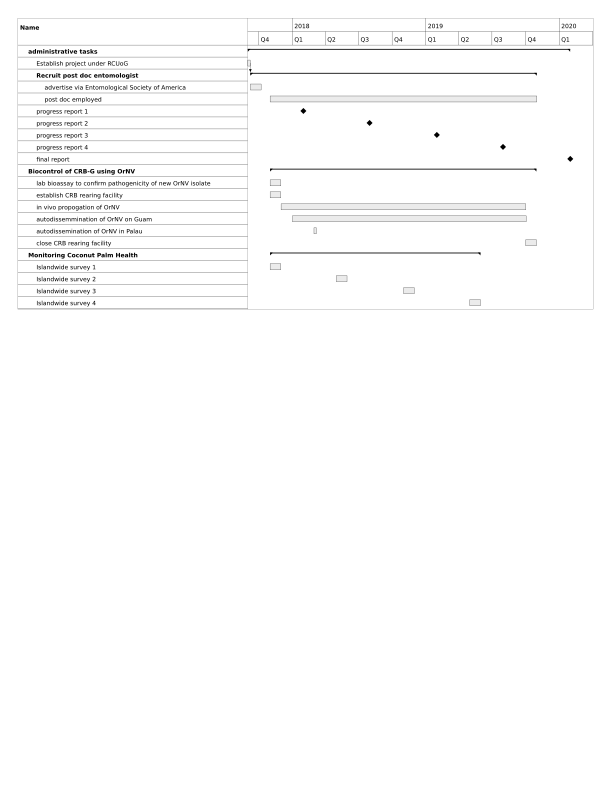
\includegraphics[width=1\textwidth,height=1\textheight,keepaspectratio]{output}.

\subsection{Potential Benefits}
\begin{itemize}
\item This project will directly benefit Guam and the Republic of Palau.
Both of these jurisdictions are infested with CRB-G. Without implementation
of effective biological control, it is likely that 50\% or more coconut
palms will be killed by CRB-G.
\item This project will indirectly benefit all other islands in Micronesia.
With very high populations of CRB-G in Gaum and the Republic of Palau,
risk of accidental introduction to other islands is extremely high.
CRB-G has already been intercepted twice on Saipan, Commonwealth of
the Northern Mariana Islands. If CRB-G infests islands and atolls
where the coconut palm as the \emph{tree of life}, islanders may have
to migrate to larger population centers.
\item Foreign exploration leading to discovery of a highly pathogenic strain
of OrNV or other microbial biocontrol agent for CRB-Guam could lead
to implementation of self sustaining population suppression and tolerable
damage levels on Guam and other islands invaded by CRB-G. 
\item Loss of 50\% or more of Guam's palms may be prevented if an effective
biocontrol agent is found and released quickly. 
\item Reduction in CRB population levels on Guam will reduce the risk of
accidental of the highly invasive CRB-Guam biotype to other Pacifc
islands and elsewhere. 
\item Development of image analysis methods may lead to a small, inexpensive,
automated CRB damage detector which could be mounted on a drone or
a conventional vehicle. This device could be used for early detection
or monitoring of CRB damage.
\end{itemize}

\section{Budget}

\begin{center}
\begin{tabular}{lr}
\hline 
\textbf{Item} & \textbf{Cost}\tabularnewline
\hline 
Personnel & \$207,170.00 \tabularnewline
Travel &  \$4,000.00 \tabularnewline
Supplies & \$15,925.00 \tabularnewline
\hline 
\textbf{SUBTOTAL} & \textbf{\$227,095.00} \tabularnewline
\hline
Administrative fee & \$22,709.50 \tabularnewline
\hline 
\textbf{TOTAL} &  \textbf{\$249,804.50} \tabularnewline
\hline 
\end{tabular} 
\par\end{center}

\begin{description}
	
\item [{Personnel}] includes salary and benefits for an insect pathologist (Dr. James Grasela, \$83,200), 
a laboratory technician (Mr. Chris Cayanan, \$60,360) and a field technician (vacant, \$60,360). Benefits for these 3 positions are calculated at 30\% * salary. The PI's salary compensation is calculated at 0.025 FTE * \$130,000.

\item [{Travel}] includes airfare and other relocation expenses for Dr. Grasela who resides in Missouri.

\item [{Supplies}] includes laboratory and insect rearing supplies (\$3,000) and fuel and maintenance for the project's field vehical (\$4,000), purchase of 150 pheromone traps (\$6,000), and purchase of 780 pheromone lures (\$2,925). 

\item [{Administrative~fee}] is equal to 10\% of the total grant award
is charged by the Research Corporation of the University of Guam for
services provided.

\end{description}

\printbibliography

\newpage{}

%\bibliographystyle{IEEEtran}
%\phantomsection\addcontentsline{toc}{section}{\refname}\bibliography{references}

\newpage{}

\appendix

\section{Supporting Technical Data}

\subsection{Self-sustaining Biological Control of CRB in Fiji Using OrNV}
\label{sub: fiji}

\begin{figure}[h]
\centering
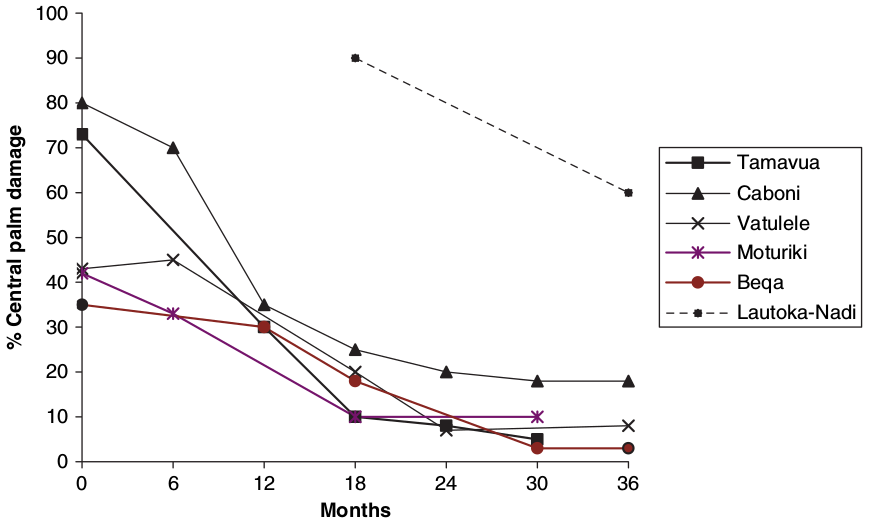
\includegraphics[width=0.7\linewidth]{images/fiji}
\caption{Reduction in coconut palm damage following release of \textit{Oryctes rhinoceros} nudivirus in Fuji. (\cite{jackson_use_2009-1})}
\label{fig:fiji}
\end{figure}

Reduction in palm damage recorded over 36 months after release of \textit{Oryctes virus} on five sites in the Fiji Islands from 1970 to 1972. No virus was released in the Lautoka area where damage remained high 18 months after the start of the program but natural incidence of disease was recorded in the area after 36 months coinciding with a decline in visible damage. Population suppression of CRB by OrNV in Fiji was still in effect 35 years after virus introduction (\cite{bedford_g._o._long-term_2013}).

\clearpage

\subsection{Automated Monitoring of CRB Damage Using Roadside Video Surveys}

\begin{figure}[h]
\centering
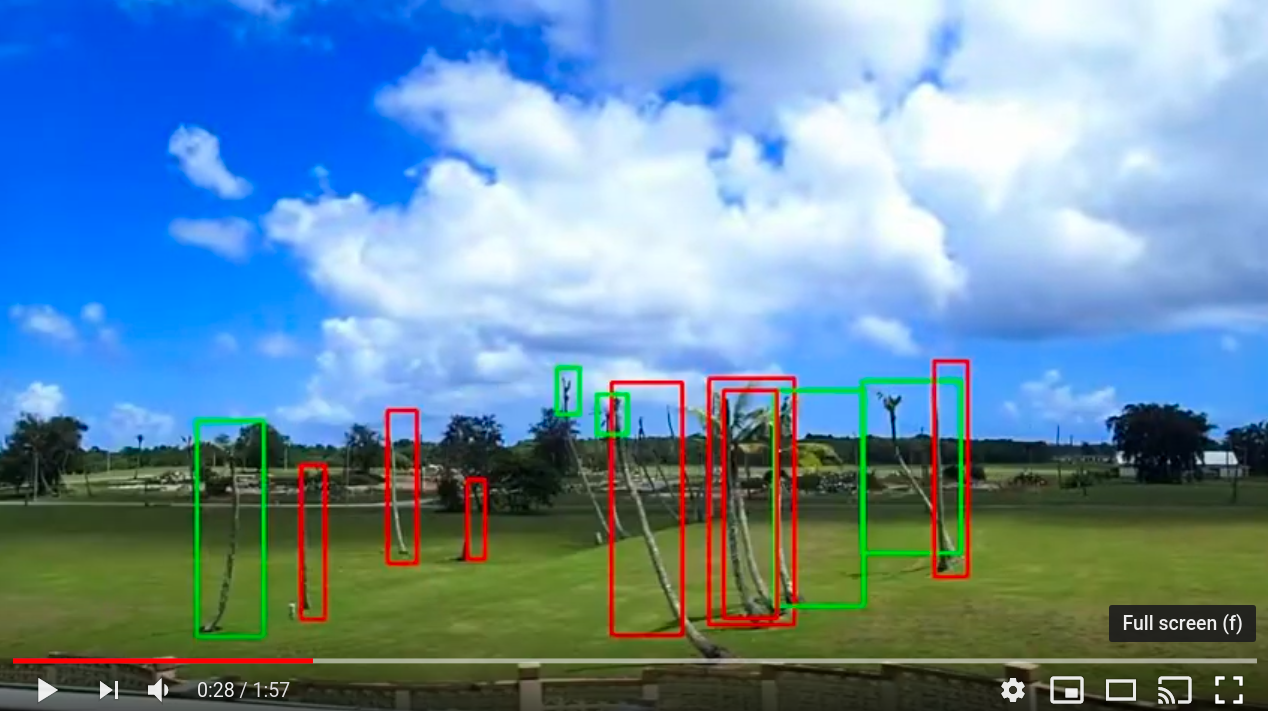
\includegraphics[width=0.7\linewidth]{images/royal-palms}
\caption{Training an Object Detector to Locate Coconut Palms Damaged or Killed by Coconut Rhinoceros Beetle. \url{https://youtu.be/zzSorqcmt9U}.}
\label{fig:royal-palms}
\end{figure}

Result of a first attempt to train an object detector (Faster R-CNN) to locate coconut trees killed or damaged by coconut rhinoceros beetle in a video. Dead palms are in red boxes, damaged palms are in green boxes. Not perfect, but it does serve as a proof of concept.

\clearpage



\section{USDA-APHIS 2020 Plant Protection Act Proposal (UNFUNDED)}
Please see next page.
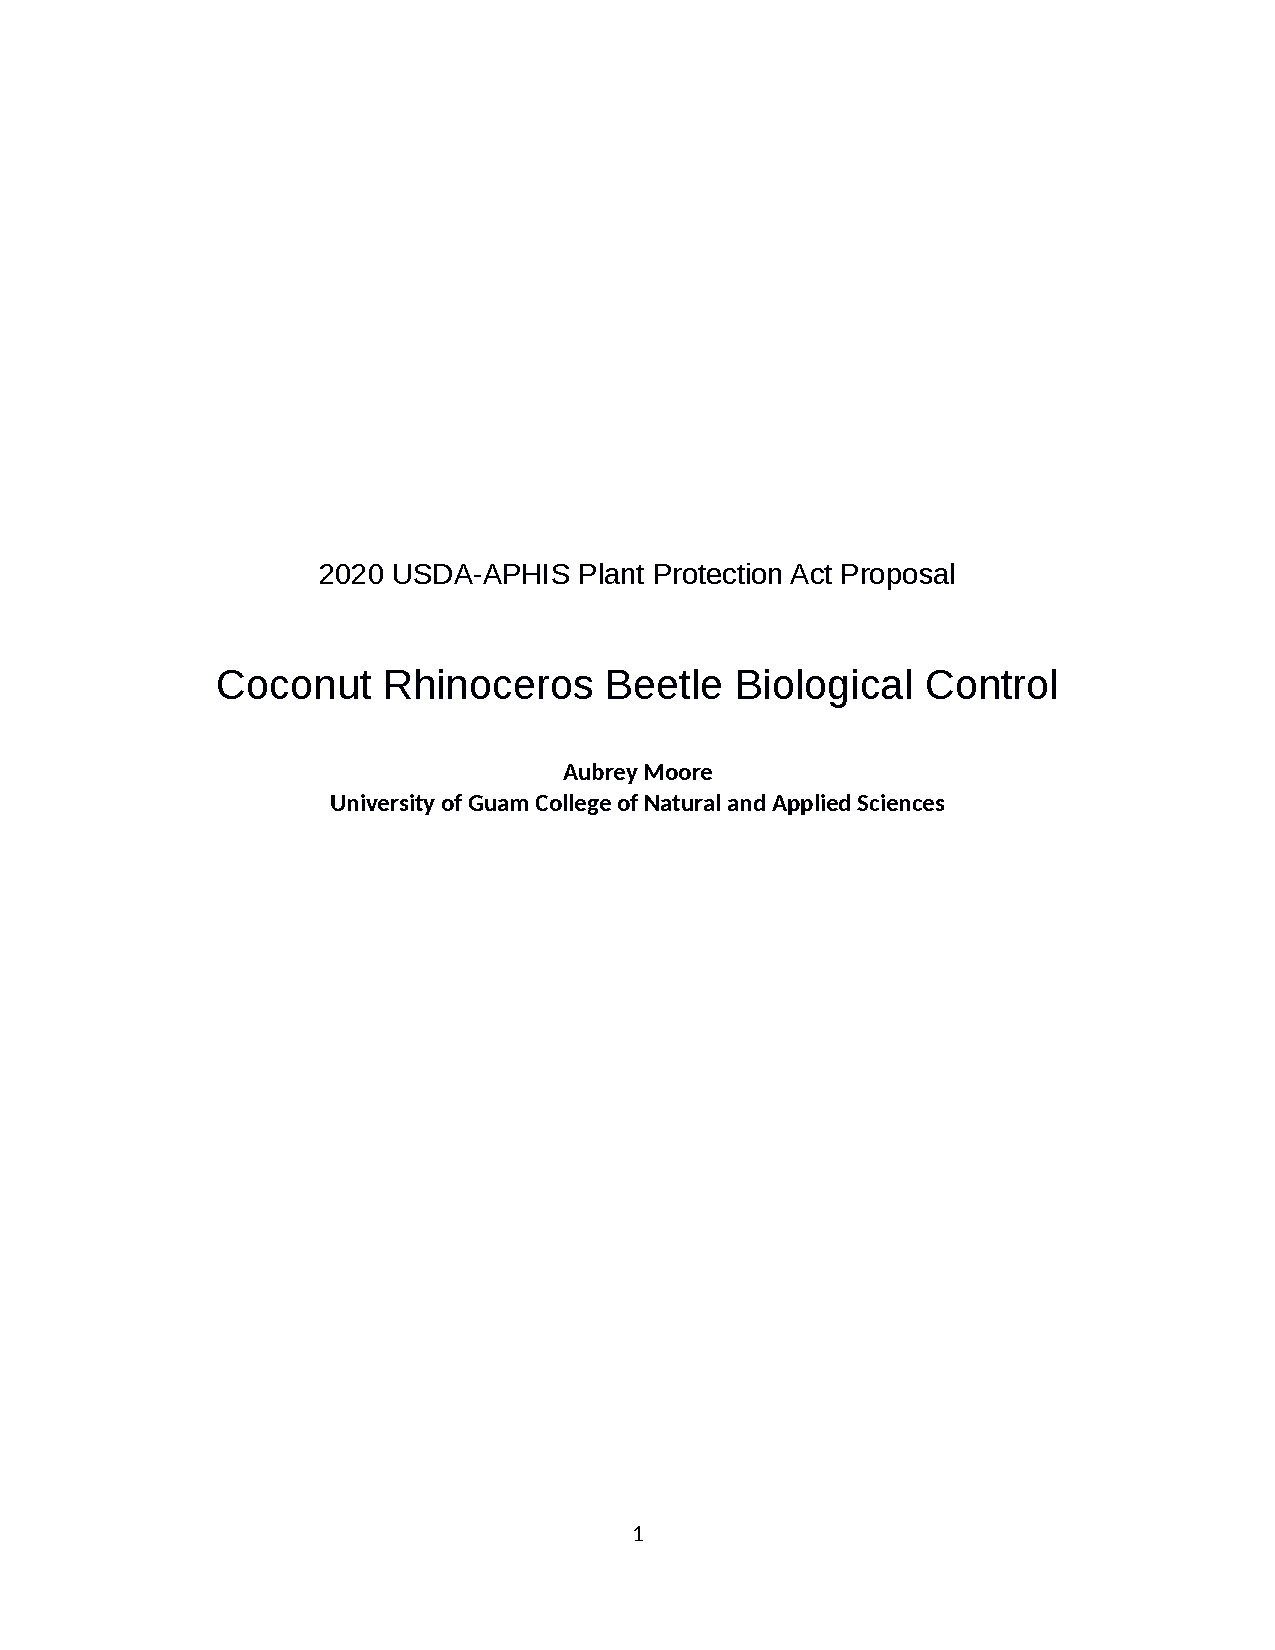
\includepdf[pages=-]{2020-PPA/Moore-FY20-PPA}

\section{DOI-OIA Grant D17AP00107 Progress Report 4}
\label{section report4}
Please see next page.
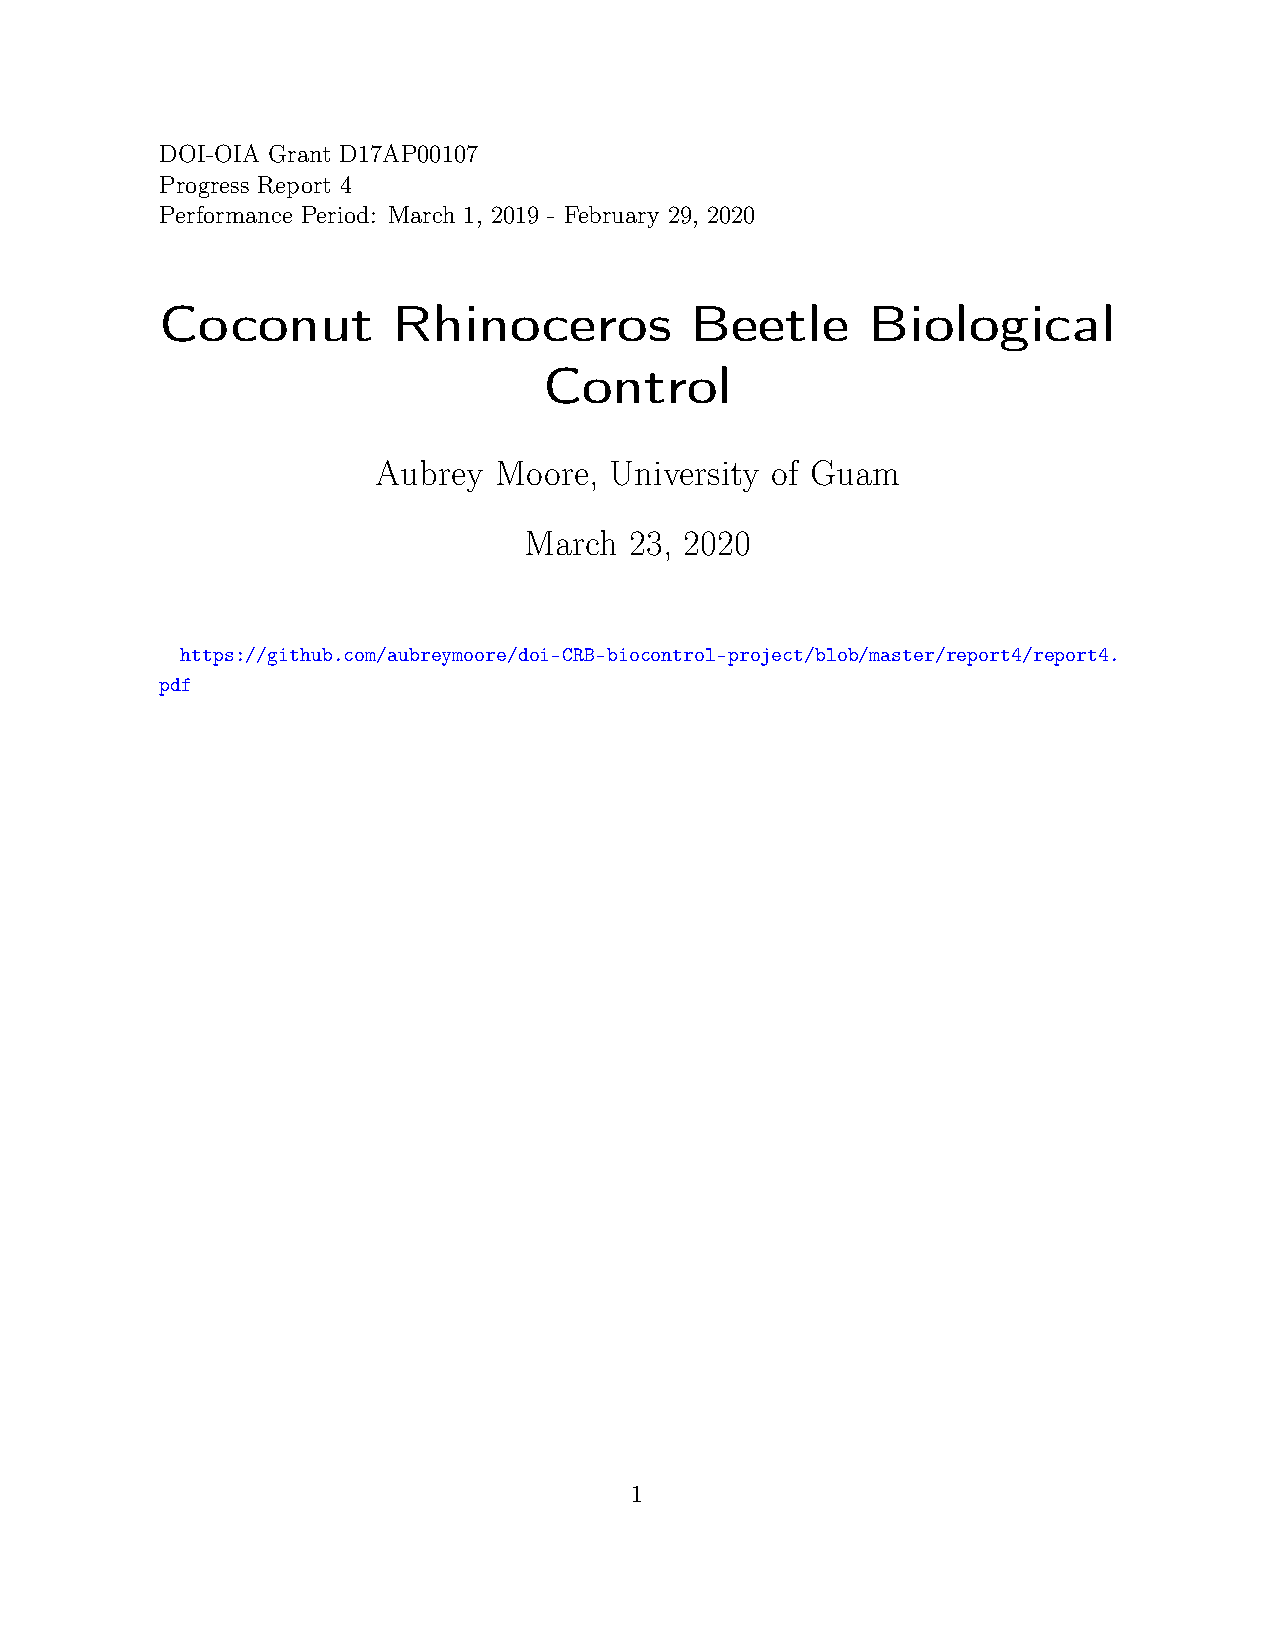
\includepdf[pages=-]{report4/report4.pdf}

\section{\label{sec:Work-Plan-for}Work Plan for CRB-G Biocontrol Project
Funded by USDA-APHIS}

\includepdf[pages=-]{\string"FY17-GU-FB-CRB biocontrol workplan\string"}

\section{\label{sec:Extracts-from-the}Extracts from the 22nd Micronesian
Islands Forum Joint Communique}

\includepdf[pages=-]{\string"extracts from MF Joint Communique\string"}

\section{Letters of Support}

\subsection{Regional Invasive Species Council}

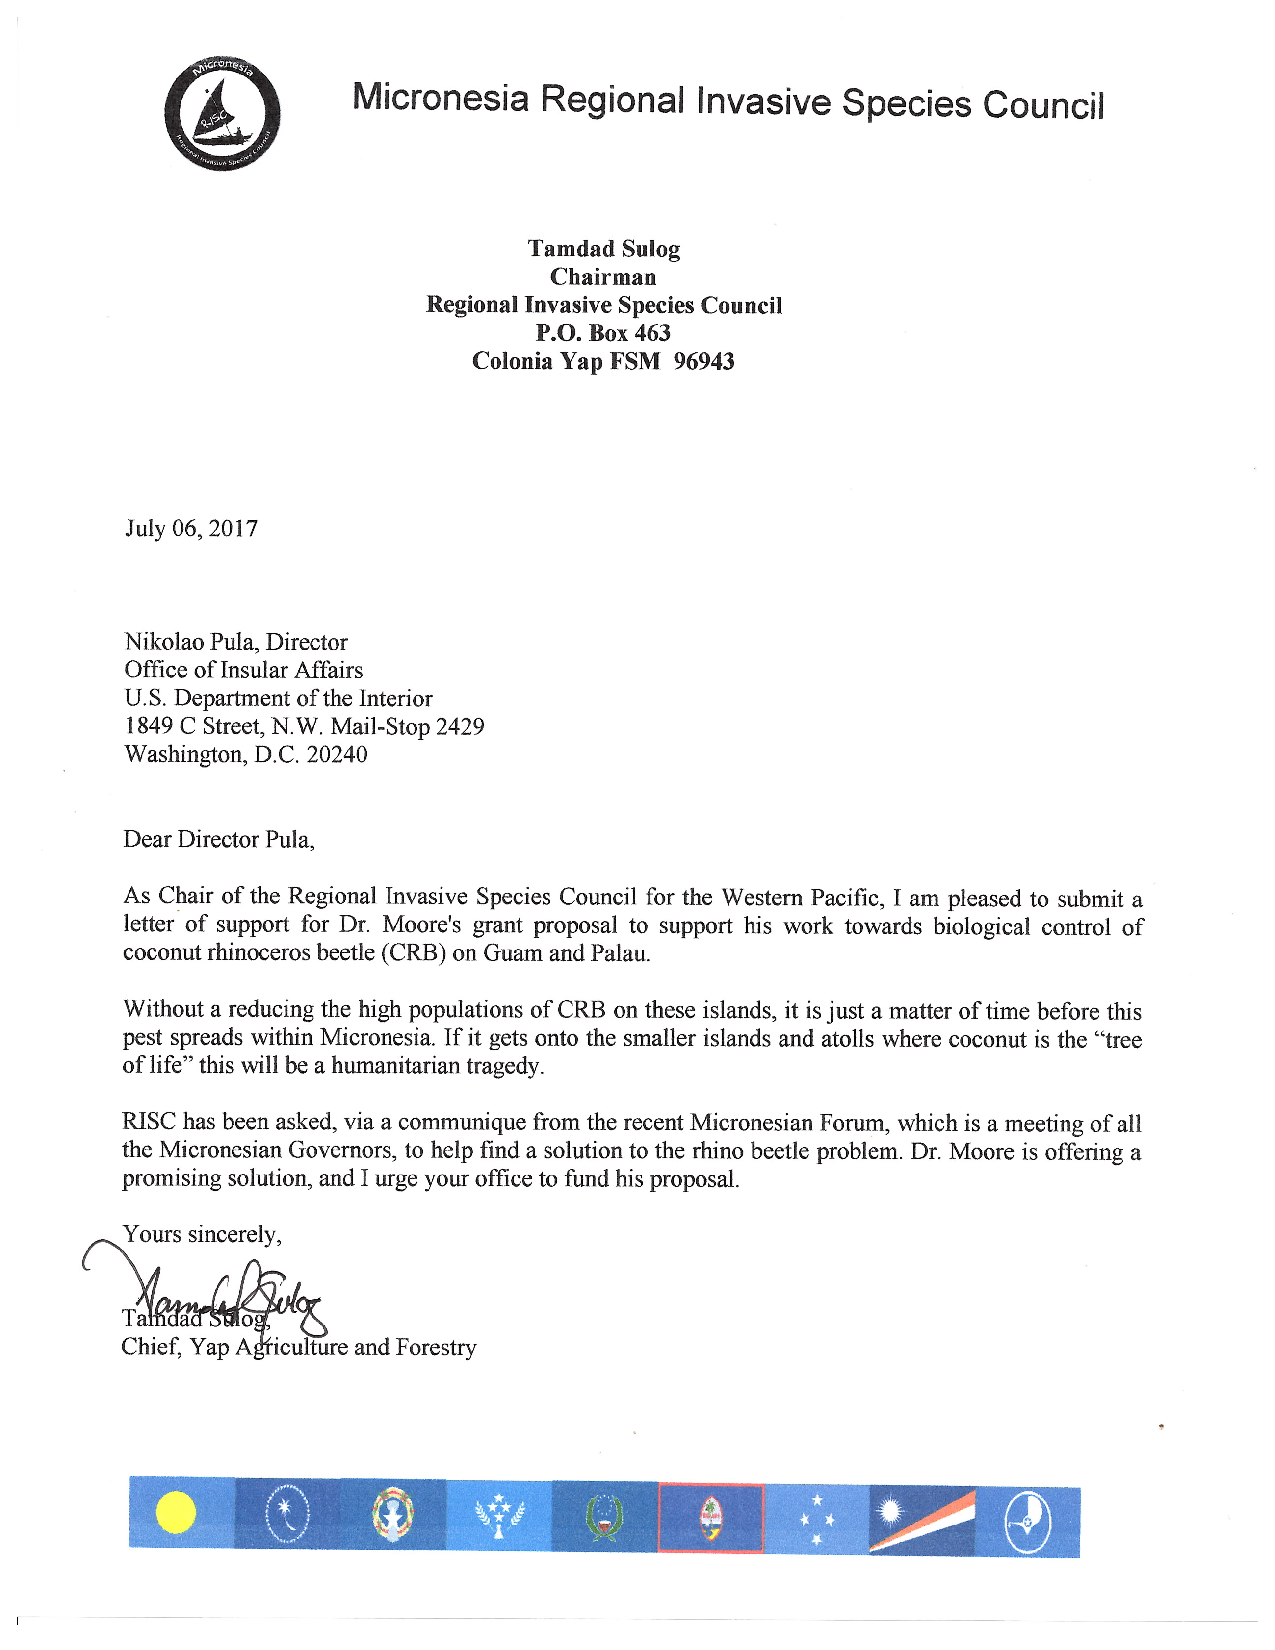
\includepdf[pages=-]{support_letters/RISC.PDF}

\subsection{Republic of Palau}

\section{Administrative Forms}

\subsection{SF-424}

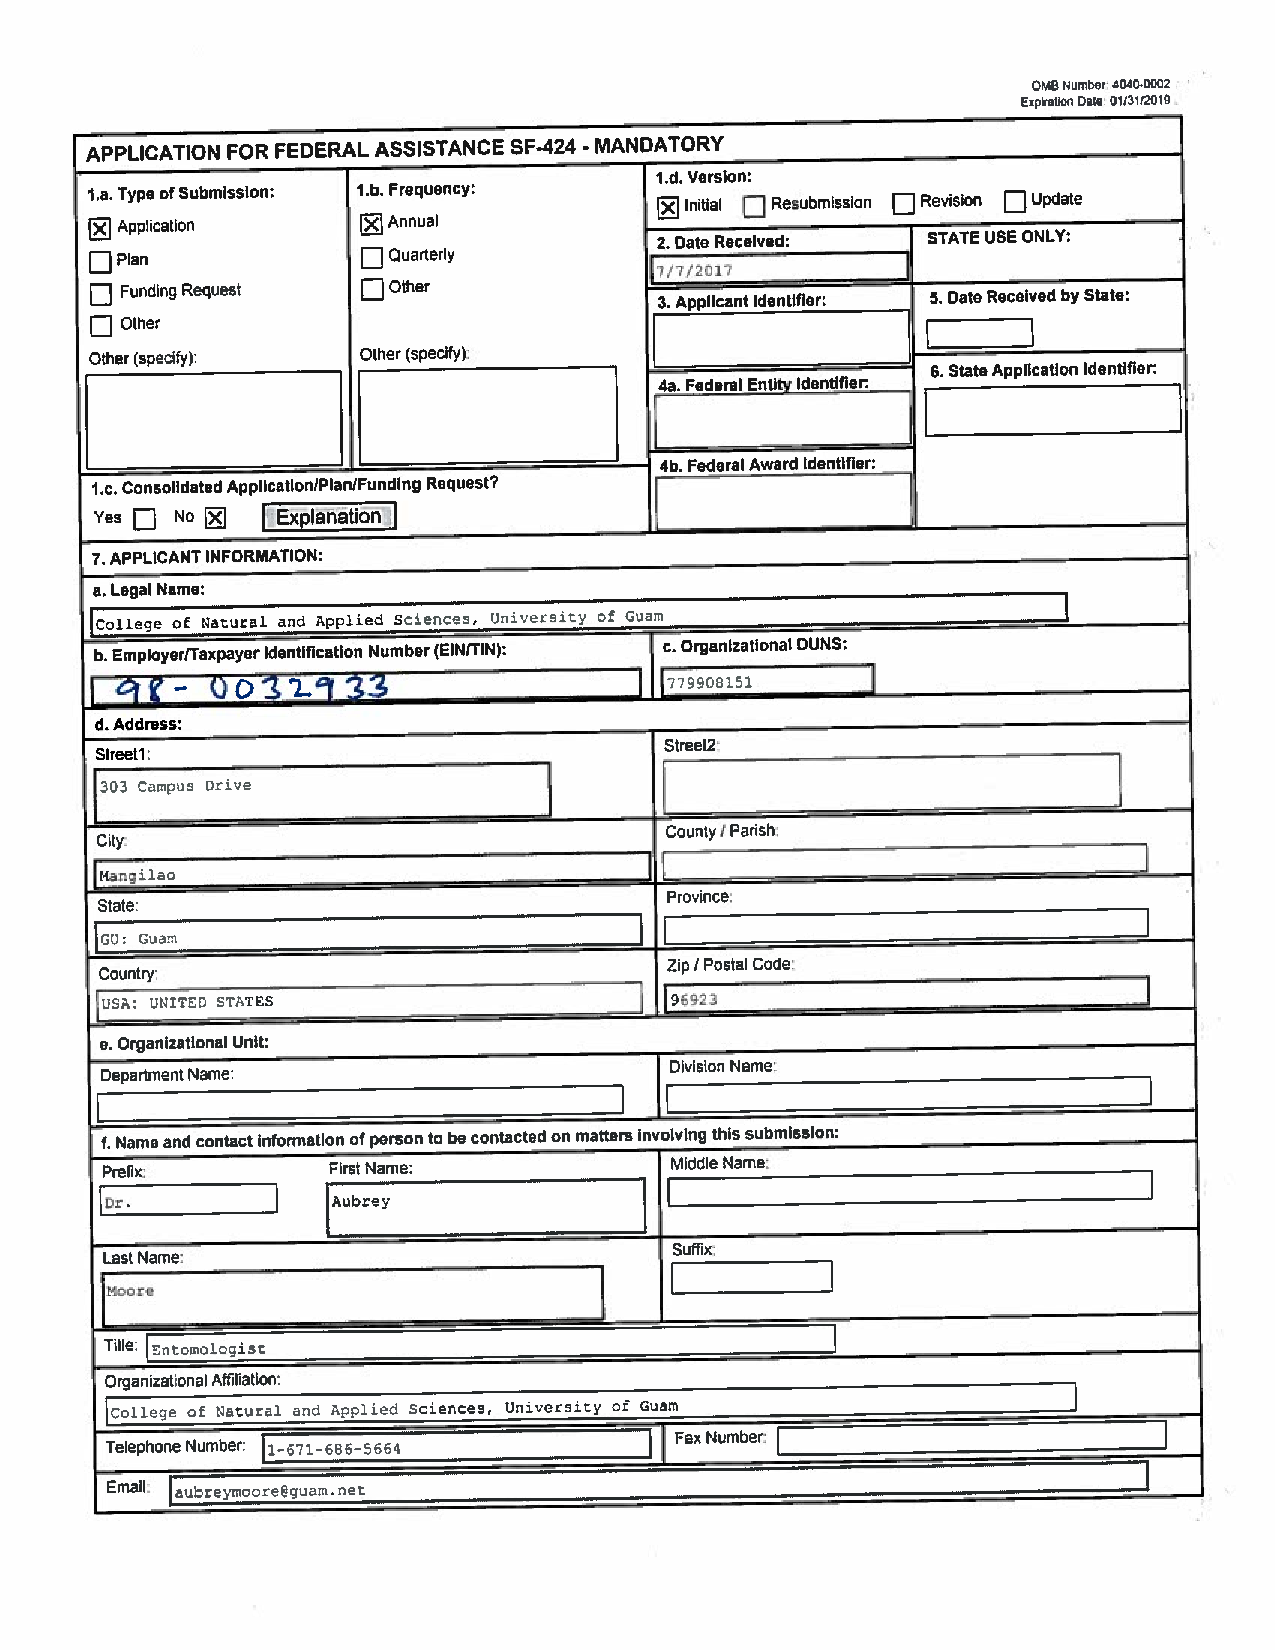
\includepdf[pages=-]{SF424_signed/SF424}

\subsection{SF-424A}

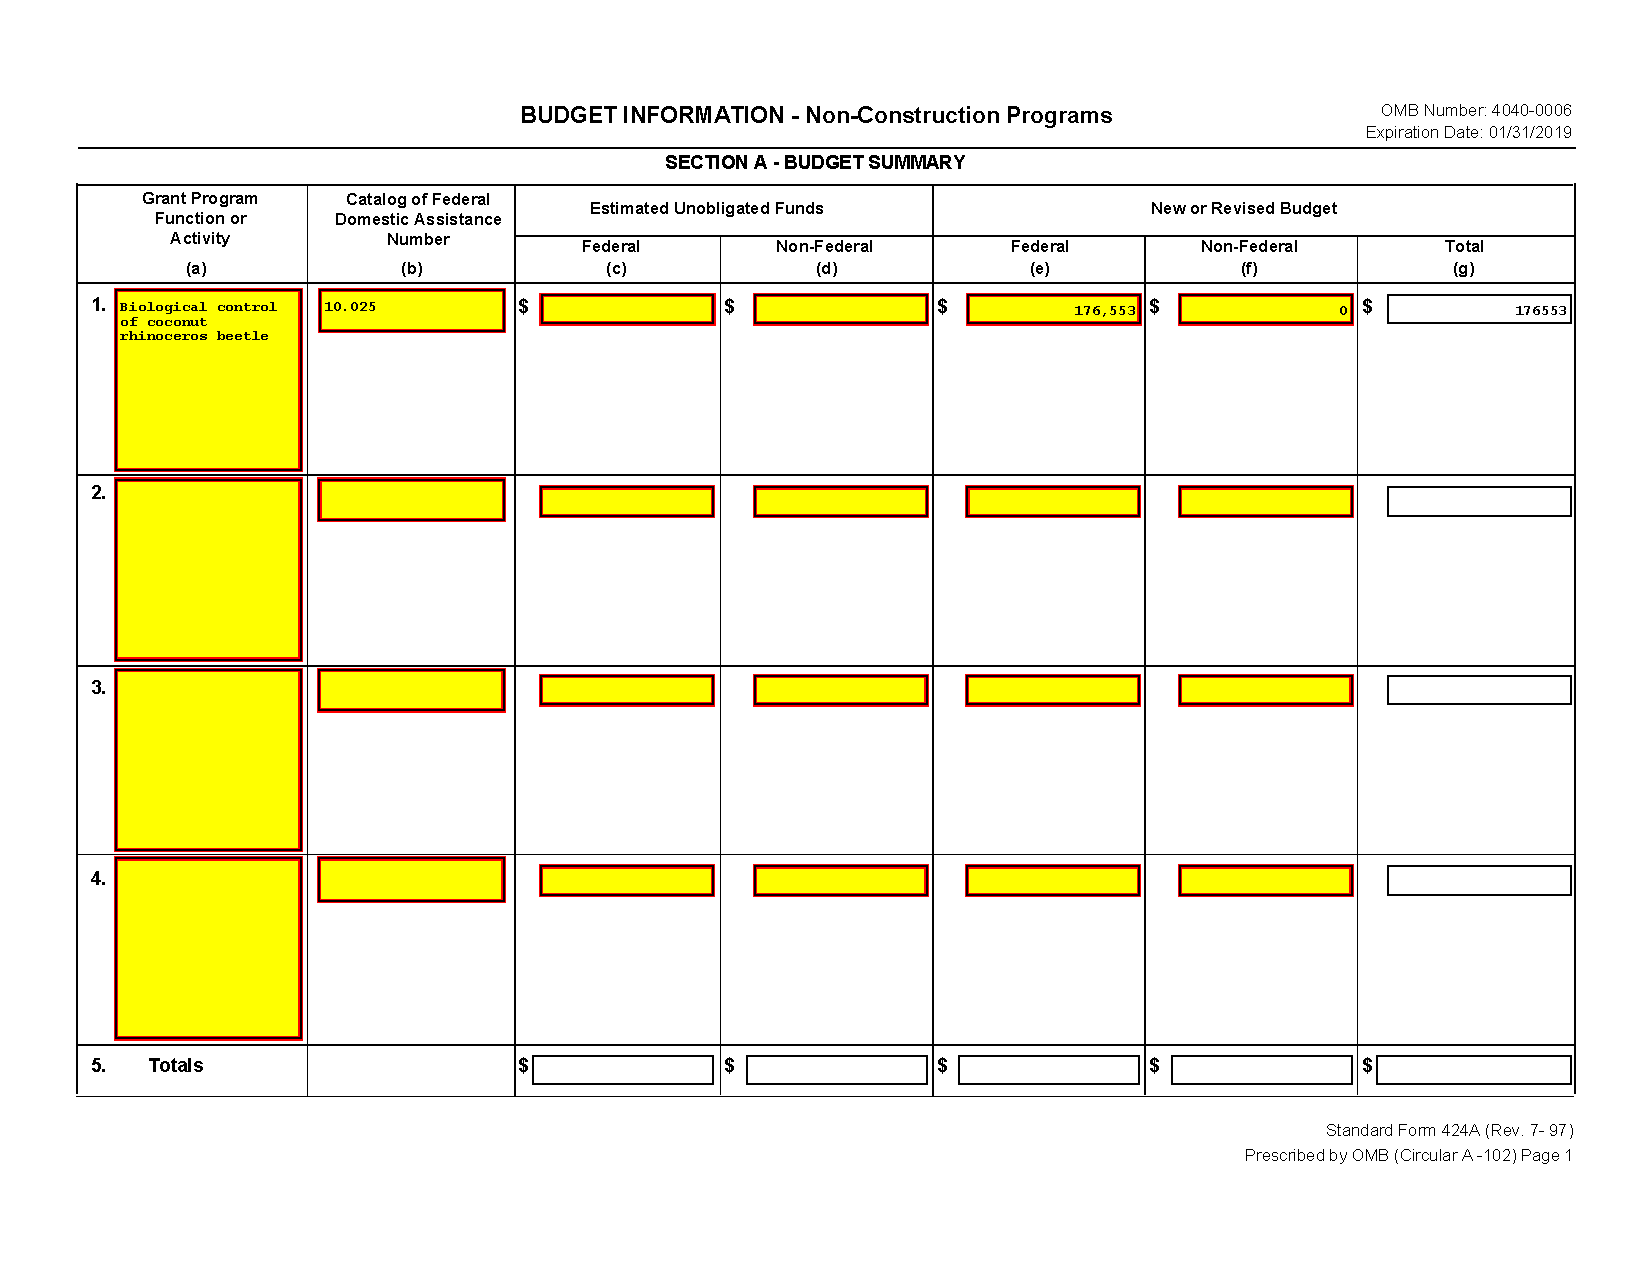
\includepdf[pages=-]{SF424_signed/SF424A}

\subsection{SF-424B}

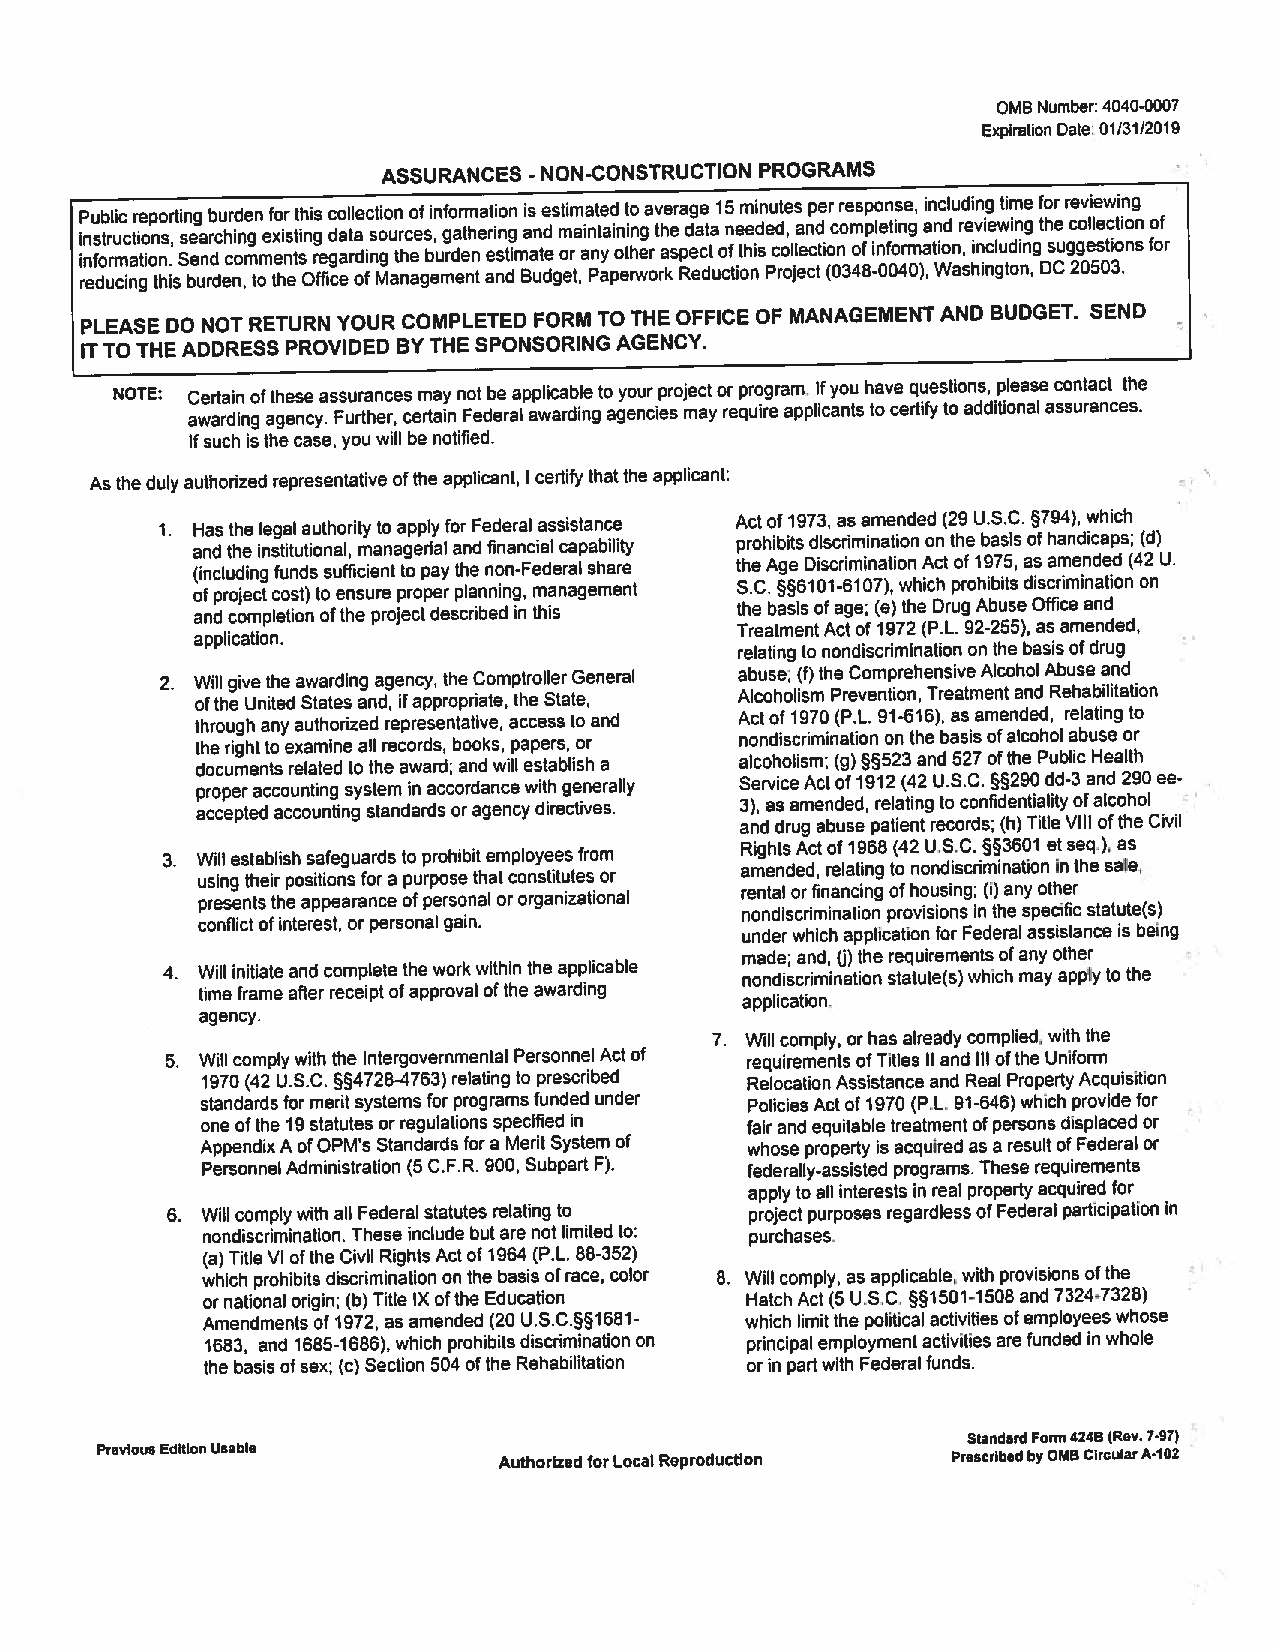
\includepdf[pages=-]{SF424_signed/SF424B}
\end{document}
